\documentclass{article}
\usepackage[margin=1in]{geometry}
\usepackage{problemset}
\showsolntrue

% Custom commands
\newcommand{\R}{\mathbb{R}}
\newcommand{\X}{\mathcal{X}}
\newcommand{\Y}{\mathcal{Y}}
\newcommand{\E}{\mathbb{E}}
\newcommand{\V}{\text{Var}}
\renewcommand{\P}{\mathbb{P}}

\begin{document}

\pstitle{%
    MATH 189%
}{
    Homework 4%
}[due Friday, February 13 at 8:00AM]

\textbf{Resources:} These problems appear in Chs. 6-7 of the textbook pgs. 283-288 and 325-329.

\textbf{Format requirements:} Type your homeworks using \LaTeX with embedded plots for the applied exercises.

\textbf{Grading:} The grading is based 50\% on completion and 50\% on correctness.
\vspace{1em}

\begin{probset}

% --- Problem 1 ---
\begin{prob}[\textbf{Ch. 6 conceptual exercise 1}]
    We perform best subset, forward stepwise, and backward stepwise selection on a single data set. For each approach, we obtain $p + 1$ models, containing 0, 1, 2, . . . , $p$ predictors. Explain your answers:

    \begin{subprobset}
        \begin{subprob}
            Which of the three models with $k$ predictors has the smallest training RSS?

            \begin{soln}
                Best subset selection will have the smallest training RSS because despite its computational cost, it will find the model with the smallest training RSS.
            \end{soln}
        \end{subprob}

        \begin{subprob}
            Which of the three models with $k$ predictors has the smallest test RSS?

            \begin{soln}
                While best subset will theoretically have the smallest training RSS, it will likely have overfit. Hence, forward and backward have a chance of having a smaller test RSS.
            \end{soln}
        \end{subprob}

        \begin{subprob}
            True or False:

            \begin{enumerate}[label=\roman*.]
                \item The predictors in the $k$-variable model identified by forward stepwise are a subset of the predictors in the $(k + 1)$-variable model identified by forward stepwise selection.
                \item The predictors in the $k$-variable model identified by backward stepwise are a subset of the predictors in the $(k + 1)$-variable model identified by backward stepwise selection.
                \item The predictors in the $k$-variable model identified by backward stepwise are a subset of the predictors in the $(k + 1)$-variable model identified by forward stepwise selection.
                \item The predictors in the $k$-variable model identified by forward stepwise are a subset of the predictors in the $(k + 1)$-variable model identified by backward stepwise selection.
                \item The predictors in the $k$-variable model identified by best subset are a subset of the predictors in the $(k + 1)$-variable model identified by best subset selection.
            \end{enumerate}

            \begin{soln}
                \begin{enumerate}[label=\roman*.]
                    \item True. We only add one predictor at a time, so the first $k$ predictors remain the same.
                    \item True. We only remove one predictor at a time, so the remaining $k$ were in the original $k+1$ predictors.
                    \item False. Not necessarily true, they could have taken different paths.
                    \item False. Not necessarily true, they could have taken different paths.
                    \item False. Not necessarily true. The best subset of $k$ predictors may be a different set than for $k+1$ predictors.
                \end{enumerate}
            \end{soln}
        \end{subprob}
    \end{subprobset}
\end{prob}

\newpage

% --- Problem 2 ---
\begin{prob}[\textbf{Ch. 6 conceptual exercise 5}]
    It is well-known that ridge regression tends to give similar coefficient values to correlated variables, whereas the lasso may give quite different coefficient values to correlated variables. We will now explore this property in a very simple setting. Suppose that $n = 2$, $p = 2$, $x_{11} = x_{12}$, $x_{21} = x_{22}$. Furthermore, suppose that $y_1 + y_2 = 0$ and $x_{11} + x_{21} = 0$ and $x_{12} + x_{22} = 0$, so that the estimate for the intercept in a least squares, ridge regression, or lasso model is zero: $\hat{\beta}_0 = 0$.

    \begin{subprobset}
        \begin{subprob}
            Write out the ridge regression optimization problem in this setting.

            \begin{soln}
                \[
                    \min_{\beta_1, \beta_2} \sum_{i=1}^2 (y_i - \beta_1 x_{i1} - \beta_2 x_{i2})^2 + \lambda (\beta_1^2 + \beta_2^2)
                \]
                where $x_{i1} = x_{i2}$ for $i = 1, 2$ (the two predictors are identical).
            \end{soln}
        \end{subprob}

        \begin{subprob}
            Argue that in this setting, the ridge coefficient estimates satisfy $\hat{\beta}_1 = \hat{\beta}_2$.

            \begin{soln}
                Since $x_{i1} = x_{i2}$ for each $i$, 
                \[
                    \min_{\beta_1, \beta_2} \sum_{i=1}^2 (y_i - (\beta_1 + \beta_2)x_{i1})^2 + \lambda (\beta_1^2 + \beta_2^2)
                \]
                First, by symmetry we can argue that $\hat{\beta}_1 = \hat{\beta}_2$. We can also argue this algebraically by finding the gradient of 
                \begin{align*}
                    \frac{\partial L}{\partial \beta_1} = 2\lambda \beta_1 - \sum_{i=1}^2 2x_{i1}(y_i - (\beta_1 + \beta_2)x_{i1}) = 0 \\
                    \frac{\partial L}{\partial \beta_2} = 2\lambda \beta_2 - \sum_{i=1}^2 2x_{i1}(y_i - (\beta_1 + \beta_2)x_{i1}) = 0
                \end{align*}
                Since they both equal 0 and the sum term is the same, we see that the minimum is achieved when $2\lambda\hat{\beta}_1 = 2\lambda\hat{\beta}_2$, so the minimum is achieved when $\hat{\beta}_1 = \hat{\beta}_2$.
            \end{soln}
        \end{subprob}

        \begin{subprob}
            Write out the lasso optimization problem in this setting.

            \begin{soln}
                \[
                    \min_{\beta_1, \beta_2} \sum_{i=1}^2 (y_i - \beta_1 x_{i1} - \beta_2 x_{i2})^2 + \lambda (|\beta_1| + |\beta_2|)
                \]
            \end{soln}
        \end{subprob}

        \begin{subprob}
            Argue that in this setting, the lasso coefficients $\hat{\beta}_1$ and $\hat{\beta}_2$ are not unique—in other words, there are many possible solutions to the optimization problem in (c). Describe these solutions.

            \begin{soln}
                The fitted value for observation $i$ is $\hat{y}_i = \beta_1 x_{i1} + \beta_2 x_{i2} = (\beta_1 + \beta_2)x_{i1}$ (since $x_{i1} = x_{i2}$). Thus the RSS depends only on $s = \beta_1 + \beta_2$, not on the individual values of $\beta_1$ and $\beta_2$. For any fixed $s$, many $(\beta_1, \beta_2)$ achieve the same fit: e.g. if $s > 0$, then $(s, 0)$, $(0, s)$, $(s/2, s/2)$ all give the same fitted values (hence same RSS) and the same penalty $|\beta_1| + |\beta_2| = s$. In fact, when $\beta_1, \beta_2 \geq 0$ and $\beta_1 + \beta_2 = s$, the penalty $|\beta_1| + |\beta_2| = s$ is constant. So the entire line segment $\{(\beta_1, \beta_2) : \beta_1 + \beta_2 = s$, $\beta_1, \beta_2 \geq 0\}$ is optimal for the chosen $s$ that minimizes the overall objective.
            \end{soln}
        \end{subprob}
    \end{subprobset}
\end{prob}

\newpage

% --- Problem 3 ---
\begin{prob}[\textbf{Ch. 7 conceptual exercise 5}]
    Consider two curves, $\hat{g}_1$ and $\hat{g}_2$, defined by 
    \begin{align*}
        \hat{g}_1 &= \arg \min_{g} \left( \sum_{i=1}^n (y_i - g(x_i))^2 + \lambda \int \left[ g^{(3)}(x) \right]^2 dx \right) \\
        \hat{g}_2 &= \arg \min_{g} \left( \sum_{i=1}^n (y_i - g(x_i))^2 + \lambda \int \left[ g^{(4)}(x) \right]^2 dx \right)
    \end{align*}
    where $g^{(m)}$ represents the $m$th derivative of $g$.

    \begin{subprobset}
        \begin{subprob}
            As $\lambda \to \infty$, will $\hat{g}_1$ or $\hat{g}_2$ have the smaller training RSS?

            \begin{soln}
                As $\lambda \to \infty$, the penalty term will dominate the RSS term. This implies that $g^{(3)}(x) \approx 0$ and $g^{(4)}(x) \approx 0$ which implies that $\hat{g}_1$ is roughly quadratic and $\hat{g}_2$ is roughly cubic. Since the cubic curve is more flexible, $\hat{g}_2$ will have the smaller training RSS.
            \end{soln}
        \end{subprob}

        \begin{subprob}
            As $\lambda \to \infty$, will $\hat{g}_1$ or $\hat{g}_2$ have the smaller test RSS?

            \begin{soln}
                Using the same logic as part (a), $\hat{g}_2$ will tend to have the smaller test RSS though this may depend on the data.
            \end{soln}
        \end{subprob}

        \begin{subprob}
            For $\lambda = 0$, will $\hat{g}_1$ or $\hat{g}_2$ have the smaller training and test RSS?

            \begin{soln}
                For $\lambda = 0$, the Losses are identical so both will have the same training and test RSS.
            \end{soln}
        \end{subprob}
    \end{subprobset}
\end{prob}

\newpage

% --- Problem 4 ---
\begin{prob}[\textbf{Ch. 6 applied exercise 9, with part (f) removed.}]
    In this exercise, we will predict the number of applications received using the other variables in the College data set.

    \begin{verbatim}
from sklearn.model_selection import train_test_split
from sklearn.linear_model import LinearRegression, RidgeCV, LassoCV
from sklearn.model_selection import GridSearchCV
from sklearn.preprocessing import StandardScaler
from sklearn.pipeline import Pipeline
from sklearn.decomposition import PCA

from sklearn.metrics import mean_squared_error
import numpy as np

from ISLP import load_data

College = load_data('College')
    \end{verbatim}

    \begin{subprobset}
        \begin{subprob}
            Split the data set into a training set and a test set.

            \begin{verbatim}
X = College.select_dtypes(include=[np.number]).drop("Apps", axis=1)
y = College['Apps']

X_train, X_test, y_train, y_test = train_test_split(X, y, test_size=0.2, random_state=1)
            \end{verbatim}
        \end{subprob}

        \begin{subprob}
            Fit a linear model using least squares on the training set, and report the test error obtained.

            \begin{verbatim}
model = LinearRegression()
model.fit(X_train, y_train)

y_pred = model.predict(X_test)
mean_squared_error(y_test, y_pred)
            \end{verbatim}

            \begin{soln}
                The test error obtained is 691695.2291394008.
            \end{soln}
        \end{subprob}

        \begin{subprob}
            Fit a ridge regression model on the training set, with $\lambda$ chosen by cross-validation. Report the test error obtained.

            \begin{verbatim}
pipeline = Pipeline([
    ('scaler', StandardScaler()),
    ('model', RidgeCV(alphas=[0.01, 0.1, 1, 10, 100, 1000]))
])
pipeline.fit(X_train, y_train)

y_pred = pipeline.predict(X_test)
mean_squared_error(y_test, y_pred)
            \end{verbatim}

            \begin{soln}
                The test error obtained is 691734.2183136111.
            \end{soln}
        \end{subprob}

        \newpage

        \begin{subprob}
            Fit a lasso model on the training set, with $\lambda$ chosen by cross-validation. Report the test error obtained, along with the number of non-zero coefficient estimates.

            \begin{verbatim}
pipeline = Pipeline([
    ('scaler', StandardScaler()),
    ('model', LassoCV(alphas=[0.01, 0.1, 1, 10, 100, 1000]))
])
pipeline.fit(X_train, y_train)

y_pred = pipeline.predict(X_test)
nonzero = np.sum(np.abs(pipeline['model'].coef_) > 1e-5)
mean_squared_error(y_test, y_pred), nonzero
            \end{verbatim}

            \begin{soln}
                The test error obtained is 729407.5304312743. The number of non-zero coefficient estimates is 13.
            \end{soln}
        \end{subprob}

        \begin{subprob}
            Fit a PCR model on the training set, with $M$ chosen by cross-validation. Report the test error obtained, along with the value of $M$ selected by cross-validation.

            \begin{verbatim}
pipeline = Pipeline([
    ('scaler', StandardScaler()),
    ('pca', PCA()),
    ('model', LinearRegression())
])
grid = GridSearchCV(
    pipeline, 
    param_grid={'pca__n_components': np.arange(X.shape[1]) + 1}, 
    scoring='neg_mean_squared_error'
)
grid.fit(X_train, y_train)

y_pred = grid.predict(X_test)
mean_squared_error(y_test, y_pred), grid.best_params_
            \end{verbatim}

            \begin{soln}
                The test error obtained is 691695.2291393969. The value of $M$ selected by cross-validation is 16.
            \end{soln}
        \end{subprob}

        \begin{subprob}[g]
            Comment on the results obtained. How accurately can we predict the number of college applications received? Is there much difference among the test errors resulting from these five approaches?

            \begin{soln}
                The test errors are very similar. We end up with a test MSE of around 691700 for all the methods except for the Lasso which has a slightly higher test MSE of 729407.
            \end{soln}
        \end{subprob}
    \end{subprobset}
\end{prob}

\newpage

% --- Problem 5 ---
\begin{prob}[\textbf{Ch. 7 applied exercise 11}]
    In Section 7.7, it was mentioned that GAMs are generally fit using a backfitting approach. The idea behind backfitting is actually quite simple. We will now explore backfitting in the context of multiple linear regression. Suppose that we would like to perform multiple linear regression, but we do not have software to do so. Instead, we only have software to perform simple linear regression. Therefore, we take the following iterative approach: we repeatedly hold all but one coefficient estimate fixed at its current value, and update only that coefficient estimate using a simple linear regression. The process is continued until convergence—that is, until the coefficient estimates stop changing. We now try this out on a toy example.

    \begin{verbatim}
import numpy as np
import matplotlib.pyplot as plt
from sklearn.linear_model import LinearRegression
\end{verbatim}

    \begin{subprobset}
        \begin{subprob}
            Generate a response $Y$ and two predictors $X_1$ and $X_2$, with $n = 100$.

            \begin{verbatim}
X1 = np.random.normal(10, 3, 100)
X2 = np.random.normal(5, 2, 100)
e = np.random.normal(0, 1, 100)

Y = 1 + 2 * X1 + 3 * X2 + e
            \end{verbatim}
        \end{subprob}

        \begin{subprob}
            Write a function \texttt{simple\_reg()} that takes two arguments \texttt{outcome} and \texttt{feature}, fits a simple linear regression model with this outcome and feature, and returns the estimated intercept and slope.

            \begin{verbatim}
def simple_reg(outcome, feature):
    model = LinearRegression()
    model.fit(feature.reshape(-1, 1), outcome)
    return model.coef_[0], model.intercept_
            \end{verbatim}
        \end{subprob}

        \begin{subprob}
            Initialize $\beta_1$ to take on a value of your choice. It does not matter what value you choose.

            \begin{verbatim}
B1 = 0
            \end{verbatim}
        \end{subprob}

        \begin{subprob}
            Keeping $\beta_1$ fixed, use your function \texttt{simple\_reg()} to fit the model:
            $Y - \beta_1 X_1 = \beta_0 + \beta_2 X_2 + \epsilon$.
            Store the result as $\beta_0$ and $\beta_2$.

            \begin{verbatim}
B2, B0 = simple_reg(Y - B1 * X1, X2)
            \end{verbatim}
        \end{subprob}

        \begin{subprob}
            Keeping $\beta_2$ fixed, fit the model:
            $Y - \beta_2 X_1 = \beta_0 + \beta_1 X_2 + \epsilon$.
            Store the result as $\beta_0$ and $\beta_1$ (overwriting their previous values).

            \begin{verbatim}
B1, B0 = simple_reg(Y - B2 * X2, X1)
            \end{verbatim}
        \end{subprob}

        \newpage

        \begin{subprob}
            Write a for loop to repeat (c) and (d) 1,000 times. Report the estimates of $\beta_0$, $\beta_1$, and $\beta_2$ at each iteration of the for loop. Create a plot in which each of these values is displayed, with $\beta_0$, $\beta_1$, and $\beta_2$.

            \begin{verbatim}
B0s, B1s, B2s = [B0], [B1], [B2]
for i in range(1000):
    B2, B0 = simple_reg(Y - B1 * X1, X2)
    B1, B0 = simple_reg(Y - B2 * X2, X1)
    B0s.append(B0)
    B1s.append(B1)
    B2s.append(B2)

plt.plot(B0s, label='B0')
plt.plot(B1s, label='B1')
plt.plot(B2s, label='B2')
plt.legend()
plt.show()
B0s[-1], B1s[-1], B2s[-1]
            \end{verbatim}

            \begin{soln}
                \begin{center}
                    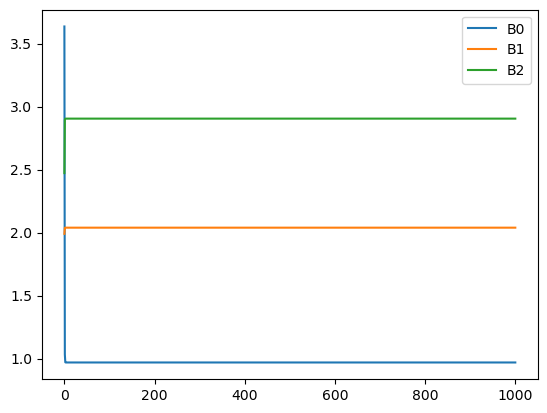
\includegraphics[width=0.8\textwidth]{Images/5f.png}
                \end{center}
                This converged really fast. The final estimates of $\beta_0$, $\beta_1$, and $\beta_2$ are 1.039, 2.039, and 2.90, respectively. which are fairly close to the true values of 1, 2, and 3, respectively.
            \end{soln}
        \end{subprob}
    \end{subprobset}
\end{prob}
\end{probset}
\end{document}